\paragraph*{Architecture}

\begin{figure}[pht]
\begin{center}
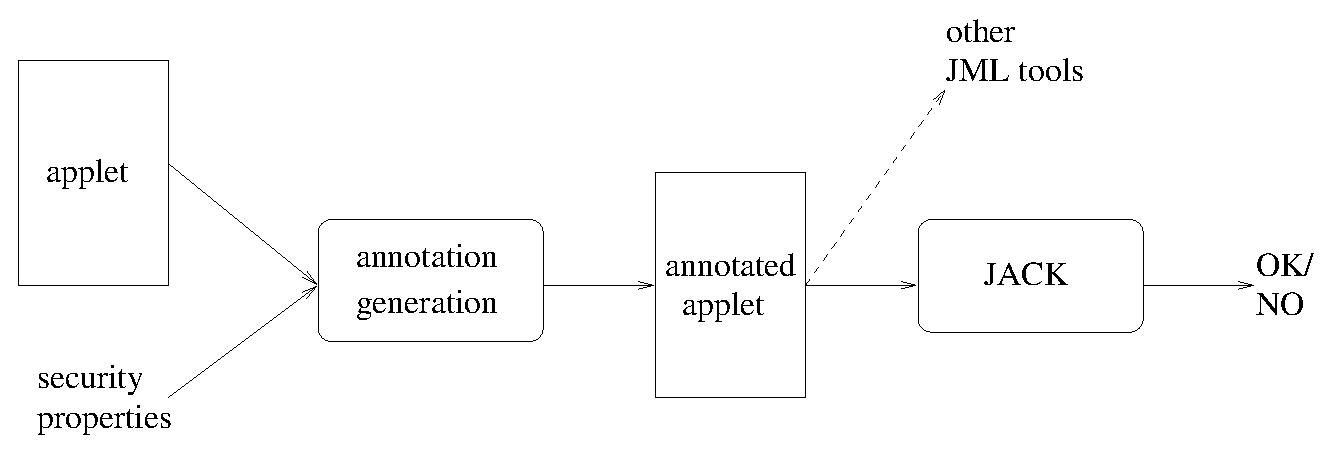
\epsfig{file=isaac/architecture.eps, width=9cm}
\end{center}
\caption{\sc Tool set for verifying high-level security properties}\label{FigArch}
\end{figure}



Figure~\ref{FigArch} shows the general architecture of the tool set
for verifying high-level security properties. Our annotation generator
can be used as a front-end for any tool accepting JML-annotated Java
(Card) applications. As input we have a security property and a Java
Card applet. The output is a JML Abstract Syntax Tree (AST), using the
format as defined for the standard JML parser. When pretty-printed,
this AST corresponds to a JML-annotated Java file. From this
annotated file, JACK generates appropriate proof obligations to check
whether the applet respects the security property.

\paragraph*{Automatic Generation of Annotations}
The purpose of this section is to provide a brief description of the
weaving phase, \emph{i.e.}~how the core-annotations are propagated
throughout the applet. We define functions \textsf{mod}, \textsf{pre},
\textsf{post} and \textsf{exc\-post}, propagating assignable clauses,
preconditions, postconditions and exceptional postconditions,
respectively. These functions have been defined and implemented for
the full Java Card language, but to present our ideas, we only give
the definitions for a representative subset of statements: statement
composition, method calls, conditional and \texttt{try}-\texttt{catch}
statements and special set-annotations. We assume the existence of
domains \textsf{MethName} of method names, \textsf{Stmt} of Java Card
statements, \textsf{Expr} of Java Card expressions, and \textsf{Var}
of static ghost variables, and functions \textsf{call} and
\textsf{body}, denoting a method call and body, respectively.

All functions are defined as mutual recursive functions on method
names, statements and expressions. When a method call is encountered,
the implementation will check whether annotations already have been
generated for this method (either by synthesizing or weaving). If not
it will recursively generate appropriate annotations. Java Card
applets typically do not contain (mutually) recursive method calls,
therefore this does not cause any problems. Generating appropriate
annotations for recursive methods would require more care (and in
general it might not be possible to do without any user interaction).


\paragraph{Propagation of assignable clauses}
First we define a function \textsf{mod} that propagates
assignable clauses for static ghost variables.

%Different from the standard JML set of modified variables in a method, that takes into account  both JML and 
%Java variables, we keep track only of JML ghost static variables. For our purposes this is sufficient because the generated pre- and postconditions involve only ghost variables.
\begin{definition}[\textsf{mod}]We define functions
%\[
%\begin{array}{rcl}
\(\mathsf{mod} \colon \mathsf{MethName} \rightarrow
\mathcal{P}(\mathsf{Var})\), 
\(
\mathsf{mod}  \colon  \mathsf{Stmt}   \rightarrow
\mathcal{P}(\mathsf{Var}) \), and 
\(\mathsf{mod}  \colon  \mathsf{Expr}   \rightarrow  \mathcal{P}(\mathsf{Var})\)
%\end{array}
%\]
by rules like (where \(m,n\,\colon\mathsf{MethName}\),
\(s_1,s_2\,\colon\mathsf{Stmt}\), \(c\,\colon\mathsf{Expr}\) and \(x\colon\mathsf{Var}\)):
\[
\begin{array}{rcl}
\mathsf{mod}(m) & = & \mathsf{mod}(\mathsf{body}(m)) \smallskip \\
\mathsf{mod}(s_1 \mathtt{;} s_2) & = & \mathsf{mod}(s_1) \cup \mathsf{mod}(s_2)\\
\mathsf{mod}(\mathsf{call}(n)) & = &  \mathsf{mod}(n) \\
\mathsf{mod}(\mathtt{if\:(} c \mathtt{)\:} s_1 \mathtt{\:else\:} s_2)
&=& \mathsf{mod}(c) \cup \mathsf{mod}(s_1) \cup \mathsf{mod}(s_2)\\
\mathsf{mod}(\mathtt{try\:} s_1 \mathtt{\:catch\:(} E \mathtt{)\:}
s_2) & = & \mathsf{mod}(s_1) \cup \mathsf{mod}(s_2)\\
\mathsf{mod}(\mathtt{set\:}x \mathtt{\:=\:} c) & = &  \{ x \} 
\end{array}
\]
\end{definition}


\paragraph{Propagation of preconditions}
Next, we define a function \textsf{pre} for
propagating preconditions. This function analyses a
method body in a sequential way---from beginning to end---computing
which preconditions of the methods called within the body have to be
propagated. To understand the reasoning behind the definition, we will
first look at an example. Suppose we are checking the \textbf{No
nested transactions} property for an application, which contains a
method \texttt{m}, whose only method calls are those shown, and which
does not contain any set annotations.
\begin{verbatim}
void m() { ... // some internal computations
           JCSystem.beginTransaction();
           ... // computations within transaction
           JCSystem.commitTransaction(); }
\end{verbatim}
Core-annotations are synthesised for \texttt{beginTransaction}
and \texttt{commit\-Transaction}. The annotations for
\texttt{beginTransaction} are shown below
\begin{verbatim}
/*@ requires TRANS == 0;
  @ assignable TRANS;
  @ ensures TRANS == 1; @*/
public static native void beginTransaction() 
                          throws TransactionException;
\end{verbatim}
Since the method is native, one cannot describe its body. However, if
it had been non-native, an annotation \texttt{//@ set TRANS = 1;}
would have been generated, to ensure that the method satisfies its
specification.

Likewise \texttt{commitTransaction} requires \texttt{TRANS == 1}
and ensures \texttt{TRANS == 0}. As we assume that \texttt{TRANS} is
not modified by the code that precedes the call to
\texttt{beginTransaction},  the only way the precondition of this method
can hold, is by requiring that it already holds at the moment
\texttt{m} is called. Thus, the precondition of
\texttt{beginTransaction} has to be propagated. In contrast, the
precondition for \texttt{commitTransaction} (\texttt{TRANS == 1})
has to be established by the postcondition of
\texttt{begin\-Transaction}, because the variable \texttt{TRANS} is
modified by this method. %Propagating the precondition of
%\texttt{commit\-Transaction} to the precondition of \texttt{m} would
%not help to guarantee that the precondition of
%\texttt{commitTransaction} holds. 
Thus, preconditions containing only unmodified variables should be
propagated.  Propagating pre- or postconditions can be considered as
passing on a method contract. Method bodies can only pass on contracts
for variables they do not modify; once they modify a variable it is
their duty to ensure that the necessary conditions are satisfied.

%In the definition of the function \textsf{pre} for propagating
%preconditions, we assume the existence of a function \textsf{mod}
%returning the set of static ghost variables modified by a
%statement. 
%As we are only interested in static ghost variables with
%primitive types, the definition is straightforward and it does not
%have to consider aliasing. 

We assume the existence of a domain \textsf{Pred} of predicates using
static ghost variables only, and function
\textsf{fv}, returning the set of free variables.

%We define \textsf{pre} on method names, statements and
%expressions. These definitions are mutually recursive.  Java Card
%applets typically do not contain (mutually) recursive method calls,
%therefore this does not cause any problems. Generating appropriate
%annotations for recursive methods would require more care (and in
%general it might not be possible to do without any user interaction).
%\begin{definition} [\textsf{pre\_init}]
%\[
%\begin{array}{rcl}
%\mathsf{pre\_init}& \colon & \mathsf{MethName} \rightarrow  \mathcal{P}(\mathsf{Pred})
%\end{array}
%\]
%\end{definition}
%The function $\textsf{pre\_init}$ returns the predicate that a method declaration is initialised with. Such an initialisation can be seen 
%for example as the specification added for the  ``core'' methods. It is in fact any pre- or postcondition specified for a method before applying the functions that  we define.  
\begin{definition}[\textsf{pre}]
We define
%\[
%\begin{array}{rcl}
\(\mathsf{pre} \colon \mathsf{MethName} \rightarrow
\mathcal{P}(\mathsf{Pred})\),
\( \mathsf{pre}  \colon  \mathsf{Stmt} \rightarrow
\mathcal{P}(\mathsf{Var}) \rightarrow \mathcal{P}(\mathsf{Pred}) \), and
\( \mathsf{pre}  \colon  \mathsf{Expr} \rightarrow
\mathcal{P}(\mathsf{Var}) \rightarrow \mathcal{P}(\mathsf{Pred}) \)
%\end{array}
%\]
by rules like (where \(m,n\,\colon\mathsf{MethName}\),
\(s_1,s_2\,\colon\mathsf{Stmt}\), \(c\,\colon\mathsf{Expr}\),
\(V\colon\mathcal{P}(\mathsf{Var})\) and \(x\colon\mathsf{Var}\)): 
\[
\begin{array}{rcl}
\mathsf{pre}(m) & = & \mathsf{pre}(\mathsf{body}(m), \emptyset) \smallskip\\
\mathsf{pre}(s_1 \mathtt{;} s_2, V) & = & \mathsf{pre}(s_1, V) \cup 
                                          \mathsf{pre}(s_2, V \cup \mathsf{mod}(s_1))\\

\mathsf{pre}(\mathsf{call}(n),V) & = & 
                \{ p \mid p \in \mathsf{pre}(n) \wedge 
                          (\mathsf{fv}(p) \cap V) = \emptyset\}\\
\mathsf{pre}(\mathtt{if\:(} c \mathtt{)\:} s_1 \mathtt{\:else\:} s_2, V) & = &
   \mathsf{pre}(c, V) \cup 
   \mathsf{pre}(s_1, V \cup \mathsf{mod}(c)) \cup\\
&&   \mathsf{pre}(s_2, V \cup \mathsf{mod}(c))\\
\mathsf{pre}(\mathtt{try\:} s_1 \mathtt{\:catch\:(} E \mathtt{)\:} s_2, V) & = & 
   \mathsf{pre}(s_1, V) \cup 
   \mathsf{pre}(s_2, V \cup \mathsf{mod}(s1))\\
\mathsf{pre}( \mathtt{set\:} x \mathtt{\:=\:} c) & = & \{\: \}
\end{array}
\]
\end{definition}

In the rules defining \textsf{pre} on \textsf{Stmt} and \textsf{Expr},
the second argument denotes the set of static ghost variables that have been
modified so far. When calculating the precondition for a method, we
calculate the precondition of its body, assuming that so far no variables
have been modified. For a statement composition, we first
propagate the preconditions for the first sub-statement, and then for
the second sub-statement, but taking into account the variables
modified by the first sub-statement. When propagating the preconditions
for a method call, we propagate all preconditions of the called method
that do not contain modified variables.  Since we are restricting our
annotations to expressions containing static ghost variables only, in
the rule for the conditional statement we cannot take the outcome of
the conditional expression into account. As a consequence, we
sometimes generate too strong annotations, but in practice this does
not cause problems. Moreover, it should be emphasised that this
only can make us reject correct applets, but it will never make us
accept incorrect ones.  Similarly, for the
\texttt{try}-\texttt{catch} statement, we always propagate the
precondition for the \texttt{catch} clause, without checking whether it
actually can get executed. Again, this will only make us reject
correct applets, but it will never make us accept incorrect
ones. Finally, a set annotation does not give rise to any propagated
precondition. 

Notice that by definition, we have the following property for the
function \textsf{pre} (where \(s\) is either in \textsf{Stmt} or
\textsf{Expr}, and \(V\) is a set of static ghost variables).
\[
p \in \textsf{pre}(s, V) \Leftrightarrow (p \in \textsf{pre}(s,
\emptyset) \wedge (\textsf{fv}(p) \cap V) = \emptyset)
\]

\paragraph{Propagation of postconditions}
In a similar way, we define functions \textsf{post} and
\textsf{exc\-post},  computing the
set of postconditions and exceptional postconditions that have to be
propagated for method names, statements and expressions. The main
difference with the definition of \textsf{pre} is that these functions run
through a method from the end to the beginning. Moreover, they have to
take into account the different paths through the method. For
each of these possible paths, we calculate the appropriate
(exceptional) postcondition. The overall (exceptional) postcondition
is then defined as the disjunction of the postconditions related to
the different paths through the method. 

\paragraph{Example}
For the example discussed above, our functions compute the following
annotations.

\begin{verbatim}
/*@ requires TRANS == 0;
  @ assignable TRANS;
  @ ensures TRANS == 0; @*/
void m() { 
   ... // some internal computations
  JCSystem.beginTransaction();
  ... // computations within transaction
  JCSystem.commitTransaction(); }
\end{verbatim}
This might seem trivial, but it is important to realise that similar
annotations will be generated for all methods calling
\texttt{m}, and transitively for all methods calling the methods
calling \texttt{m} \emph{etc.}
Having an algorithm to generate such annotations enables to check
automatically a large class of high-level security properties.
